\section{Experiments}\label{s:experiments}
This section describes a set of experiments to evaluate our basic
method and several extensions.
First, we compare our model with a traditional GAN for the task
of image generation and a GAN for 3D shapes.
We present quantitative and qualitative results.
Second, we demonstrate that our method is able to induce 3D shapes from
unlabeled images even when the collection contains only a single view per object.
Third, we present 3D shapes induced by our model from a variety of
categories such as airplanes, cars, chairs, motorbikes, and
vases. Using the same architecture, we show how our model is able to
induce coherent 3D shapes when the training data contains images mixed
from multiple categories.
Finally, we show applications of our method in predicting 3D shape
from a novel 2D shape, and performing shape interpolation.


\begin{figure*}[t]
\setlength{\tabcolsep}{0pt}
\centering
\begin{tabular}{cccccccc}
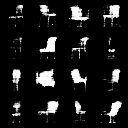
\includegraphics[width=.12\linewidth]{prgan/fig/comparison/2dgan0.png} &
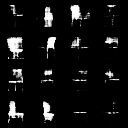
\includegraphics[width=.12\linewidth]{prgan/fig/comparison/2dgan3.png} &
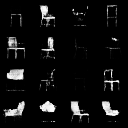
\includegraphics[width=.12\linewidth]{prgan/fig/comparison/2dgan5.png} &
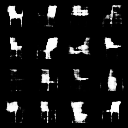
\includegraphics[width=.12\linewidth]{prgan/fig/comparison/2dgan7.png} \hfill&
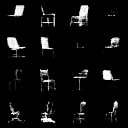
\includegraphics[width=.12\linewidth]{prgan/fig/comparison/pr2dgan4.png} &
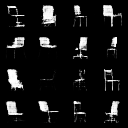
\includegraphics[width=.12\linewidth]{prgan/fig/comparison/pr2dgan5.png} &
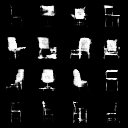
\includegraphics[width=.12\linewidth]{prgan/fig/comparison/pr2dgan6.png} &
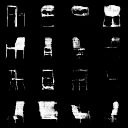
\includegraphics[width=.12\linewidth]{prgan/fig/comparison/pr2dgan3.png} \\
	\multicolumn{4}{c}{(a) Results from 2D-GAN.} \vspace{4pt} &
	\multicolumn{4}{c}{(a) Results from \prgan.} \vspace{4pt}
\end{tabular}
\caption{\label{fig:validation2} Comparison between 2D-GAN~\cite{goodfellow2014generative} and our \prgan model for image generation on the chairs dataset. Refer to Figure~\ref{fig:generate-shapes} third row, left column for samples of the input data.}
\end{figure*}

\paragraph{Input data.} We generate training images synthetically using 3D shapes available in the
ModelNet~\cite{wu20153d} and ShapeNet~\cite{chang2015shapenet} databases. Each category contains a few hundred to thousand shapes. We render each
shape from 8 evenly spaced viewing angles with orthographic projection to produce binary images. Hence our assumption is that the viewpoints of the training images (which are unknown to the network) are uniformly distributed. If we have prior knowledge about the viewpoint distribution (e.g. there may be more frontal views than side views), we can adjust the projection module to incorporate this knowledge. To reduce aliasing, we
render each image at $64\times64$ resolution and downsample to $32\times32$. We have found that this generally improves
the results. Using synthetic data allows us to easily perform controlled experiments to analyze our method. 
It is also possible to use real images downloaded from a search engine as discussed in Section \ref{s:discussion}.

\subsection{Results}
We quantitatively evaluate our model by comparing its ability to generate
2D and 3D shapes.
To do so, we use 2D image GAN similar to DCGAN~\cite{radford2015unsupervised} and a 3D-GAN
similar to the one presented in \cite{wu2016learning}.
At the time of this writing the implementation of \cite{wu2016learning} is not public yet, therefore we
implemented our own version.
We will refer to them as 2D-GAN and 3D-GAN, respectively.
The 2D-GAN has the same discriminator architecture as the \prgan, but the generator contains a sequence of 2D transposed convolutions instead of 3D ones, and
the projection module is removed.
The 3D-GAN has a discriminator with 3D convolutions instead of 3D ones.
The 3D-GAN generator is the same as the \prgan, but without the projection module.

The models used in this experiment are chairs from ModelNet dataset~\cite{wu20153d}.
From those models, we create two sets of training data: voxel grids and images.
The voxel grids are generated by densely sampling the surface and inside of each mesh, and binning the sample points into $32\times32\times32$ 
grid.
A value 1 is assigned to any voxel that contains at least one sample point, and 0 otherwise.
Notice that the voxel grids are only used to train the 3D-GAN, while the images are used to train the 2D-GAN and our \prgan.

\begin{figure*}[t]
\setlength{\tabcolsep}{0pt}
\centering
\begin{tabular}{cccc|cccc}
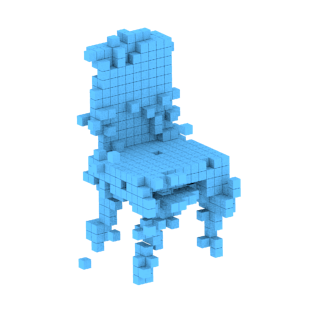
\includegraphics[width=.12\linewidth]{prgan/fig/comparison/3dgan8.png} &
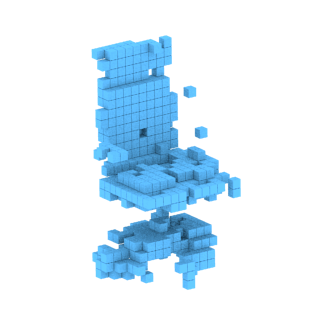
\includegraphics[width=.12\linewidth]{prgan/fig/comparison/3dgan9.png} &
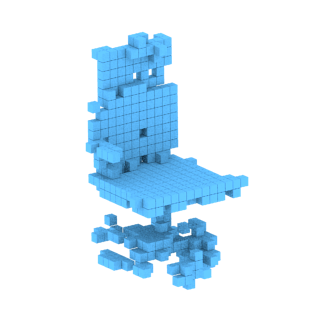
\includegraphics[width=.12\linewidth]{prgan/fig/comparison/3dgan10.png} &
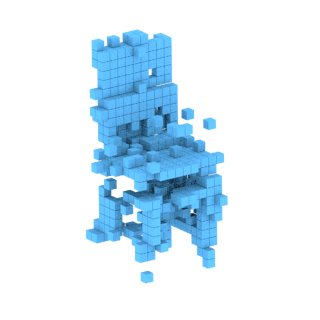
\includegraphics[width=.12\linewidth]{prgan/fig/comparison/3dgan11.png} &
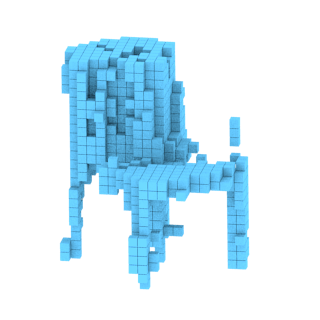
\includegraphics[width=.12\linewidth]{prgan/fig/comparison/prgan0.png} &
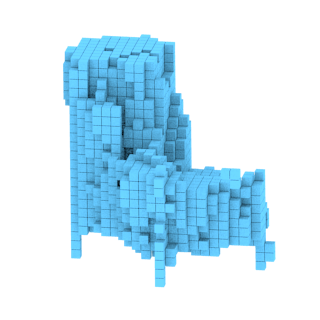
\includegraphics[width=.12\linewidth]{prgan/fig/comparison/prgan1.png} &
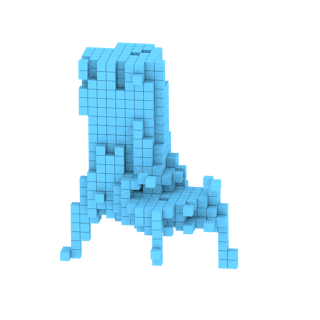
\includegraphics[width=.12\linewidth]{prgan/fig/comparison/prgan2.png} &
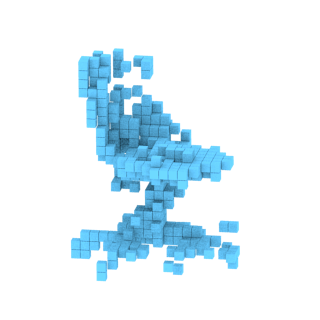
\includegraphics[width=.12\linewidth]{prgan/fig/comparison/prgan3.png} \\
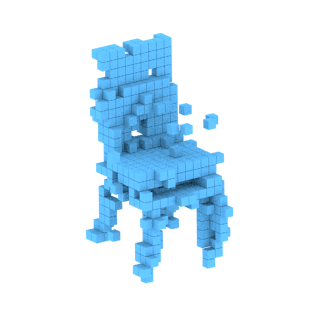
\includegraphics[width=.12\linewidth]{prgan/fig/comparison/3dgan12.png} &
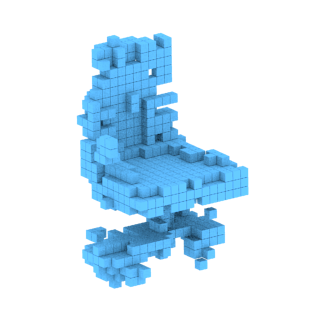
\includegraphics[width=.12\linewidth]{prgan/fig/comparison/3dgan13.png} &
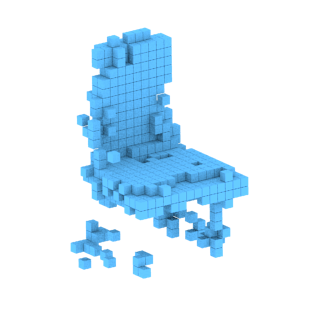
\includegraphics[width=.12\linewidth]{prgan/fig/comparison/3dgan14.png} &
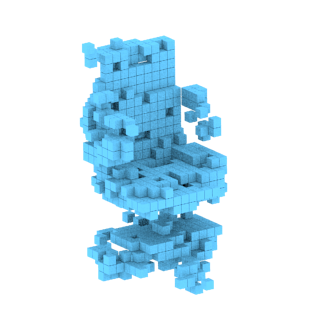
\includegraphics[width=.12\linewidth]{prgan/fig/comparison/3dgan15.png} &
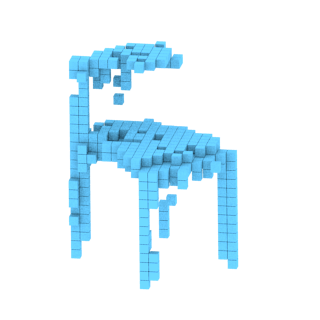
\includegraphics[width=.12\linewidth]{prgan/fig/comparison/prgan4.png} &
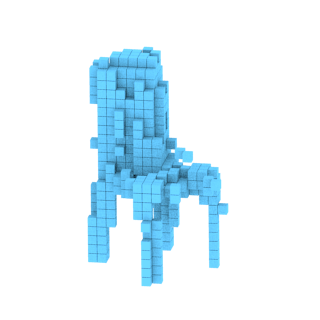
\includegraphics[width=.12\linewidth]{prgan/fig/comparison/prgan5.png} &
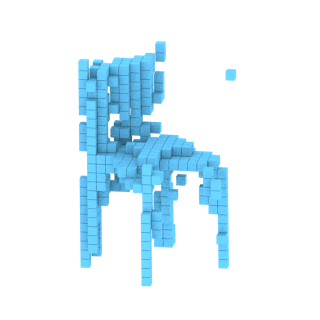
\includegraphics[width=.12\linewidth]{prgan/fig/comparison/prgan6.png} &
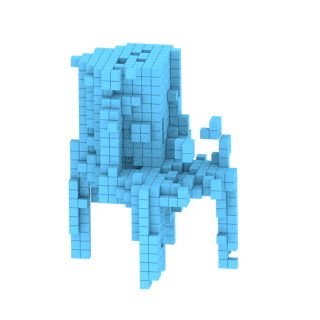
\includegraphics[width=.12\linewidth]{prgan/fig/comparison/prgan7.png} \\
\multicolumn{4}{c}{(a) Results from 3D-GAN.} &
\multicolumn{4}{c}{(a) Results from \prgan.}\\
\end{tabular}
\caption{\label{fig:validation3} Comparison between 3D-GAN~\cite{wu2016learning} and our \prgan for 3D shape generation. The 3D-GAN is trained on 3D voxel representation of the chair models, and the \prgan is trained on images of the chair models (refer to Figure~\ref{fig:generate-shapes} third row).}
\end{figure*}

Our quantitative evaluation is done by taking the Maximum Mean Discrepancy (MMD)~\cite{gretton2006kernel} 
between the data created by the generative models and the training data.
We use a kernel bandwidth of $10^{-3}$ for images and $10^{-2}$ for voxel grids.
The training data consists of 989 voxel grids and 7912 images.
To compute the MMD, we draw 128 random data points from each one of the generative models.
The distance metric between the data points is the hamming distance divided by the dimensionality of the data.
Because the data represents continuous occupancy values, we binarize them by using a threshold of $0.001$ for images or voxels created
by \prgan, and $0.1$ for voxels created by the 3D-GAN.

\begin{figure}[t]
\centering
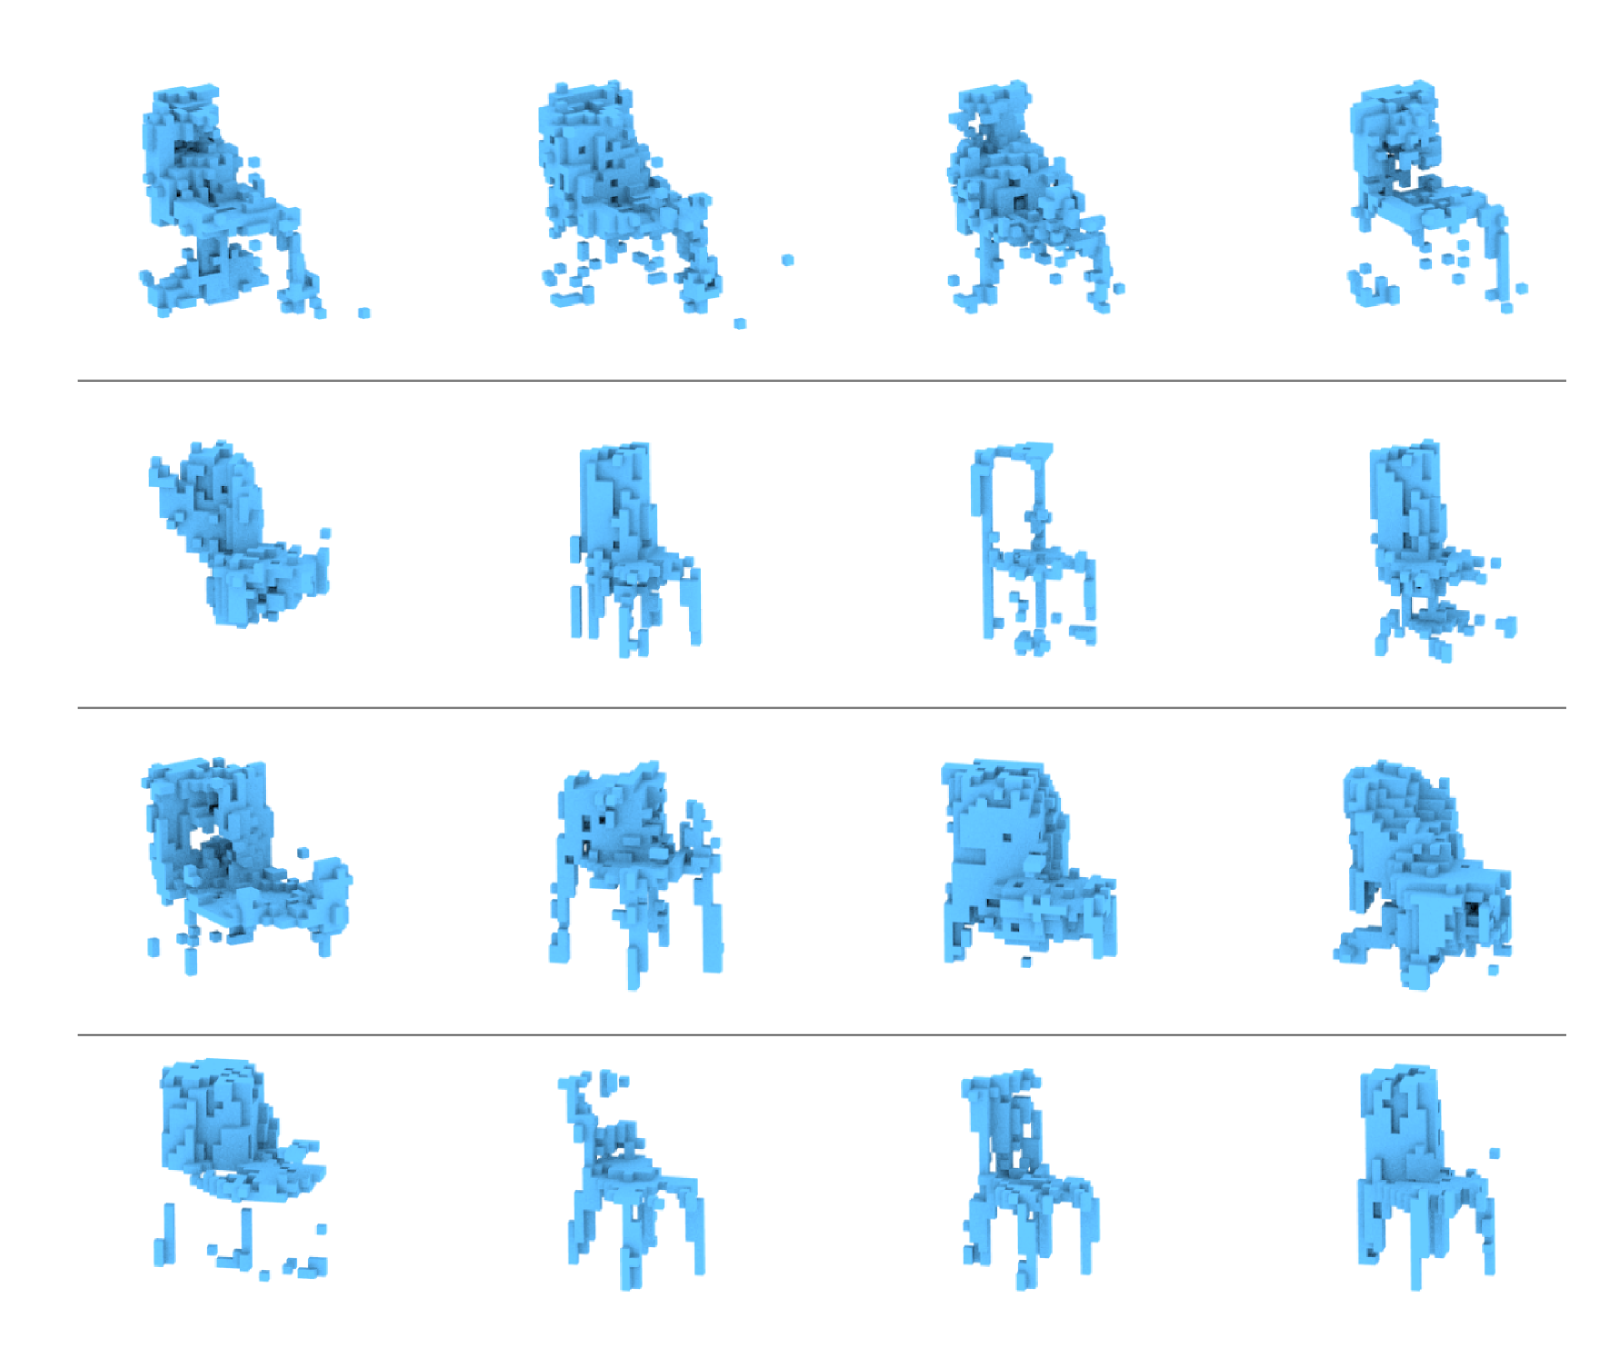
\includegraphics[width=0.75\linewidth]{prgan/fig/varying_views.png}
\caption{\label{fig:varying_views} Shapes generated from \prgan by varying the number of views per object in the training data. From the top row to the bottom row, the number of views per object in the training set are 1, 2, 4, and 8 respectively.}
\vspace{-8pt}
\end{figure}

Results show that for 2D-GAN, the MMD between the generated images and the training data is \textbf{90.13}. For \prgan, the MMD is \textbf{88.31}, which is slightly better quantitatively than 2D-GAN. Figure~\ref{fig:validation2} shows a qualitative comparison. The results are visually very similar. For 3D-GAN, the MMD between the generated voxel grids and the training voxel grids is \textbf{347.55}. For \prgan, the MMD is \textbf{442.98}, which is worse compared to 3D-GAN. This is not surprising as 3D-GAN is trained on 3D data, while \prgan is trained on the image views only. Figure~\ref{fig:validation3} presents a qualitative comparison. In general \prgan has trouble generating interior structures because the training images are binary, carry no shading information, and are taken from a limited set of viewing angles. Nonetheless, it learns to generate exterior structures reasonably well.



\subsubsection{Varying the number of views per model} 
In the default setting, our training data is generated by sampling 8 views per
object. 
Note that we do not provide the association between views and instances
to the generator.
Here we study the ability of our method in the more challenging case
where the training data contains fewer number of views per object. 
To do so, we generate a new training set that contains only 1 randomly
chosen view per object and use it to train \prgan. We then repeat the
experiments for 2 randomly chosen views per object, and also 4. The
results are shown in Figure~\ref{fig:varying_views}. 
Notice that the 3D shapes generated by \prgan become slightly better as the number of views
increase. 
An interesting question is what's the root cause for such improvements -- it may be due to the fact 
that more training data is available as the number of views per object increases; or it could be that the presence of multiple views of the same object lead to better reconstruction.
Thus we further investigate this question by performing an additional experiment, where the training data consists of 8 views per instance, but only using half of the instances available in the dataset.
In other words, this setup has the same number of images as the experiment with 4 views of all instances,
which makes them comparable in terms of the total amount of training data.
We observed no qualitative or quantitative difference in the objects generated in these two scenarios.
Quantitative results using the model and metrics described in Section~\ref{s:discussion} are shown
in Table~\ref{tab:newcomp}.
Therefore, we believe the improved quality is most likely a consequence of extra data available during training.
Nevertheless, it is important to highlight that differently from other approaches that require object correspondence~\cite{yan2016perspective,mvcTulsiani18}
our method is able to induce reasonable shapes, even in the case of a single view per object.







\begin{figure}[t]
\setlength{\tabcolsep}{0pt}
\begin{tabular}{cccccc}
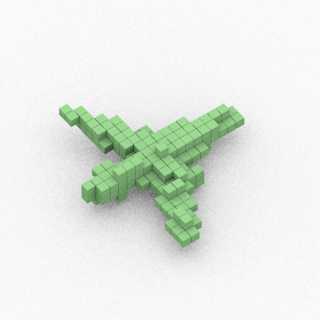
\includegraphics[width=.166\linewidth]{prgan/fig/interpolation/ap0.png} &
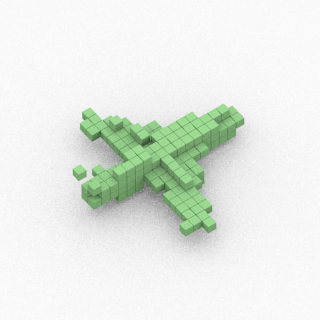
\includegraphics[width=.166\linewidth]{prgan/fig/interpolation/ap1.png} &
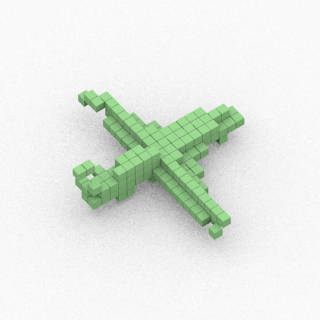
\includegraphics[width=.166\linewidth]{prgan/fig/interpolation/ap3.png} &
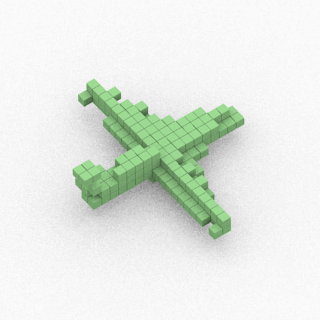
\includegraphics[width=.166\linewidth]{prgan/fig/interpolation/ap4.png} &
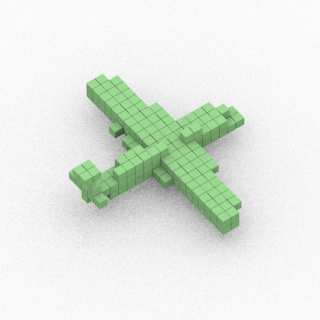
\includegraphics[width=.166\linewidth]{prgan/fig/interpolation/ap6.png} &
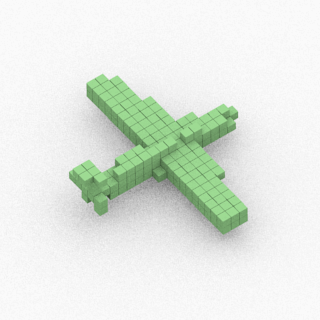
\includegraphics[width=.166\linewidth]{prgan/fig/interpolation/ap7.png} \\
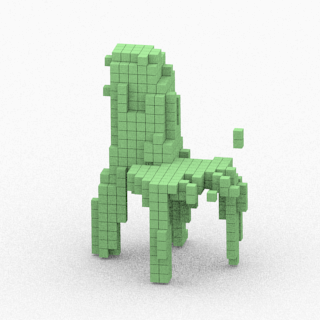
\includegraphics[width=.166\linewidth]{prgan/fig/interpolation/ch0.png} &
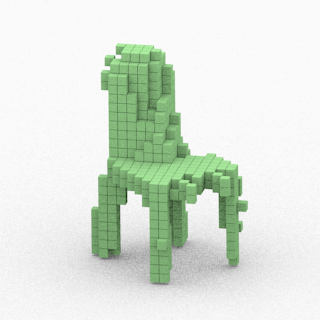
\includegraphics[width=.166\linewidth]{prgan/fig/interpolation/ch3.png} &
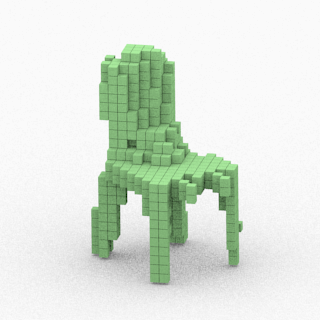
\includegraphics[width=.166\linewidth]{prgan/fig/interpolation/ch4.png} &
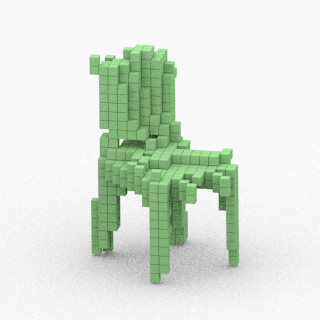
\includegraphics[width=.166\linewidth]{prgan/fig/interpolation/ch5.png} &
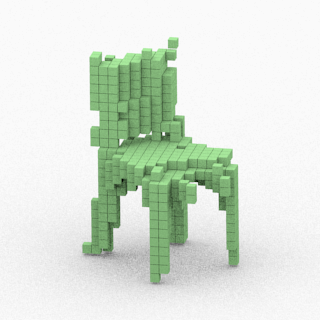
\includegraphics[width=.166\linewidth]{prgan/fig/interpolation/ch6.png} &
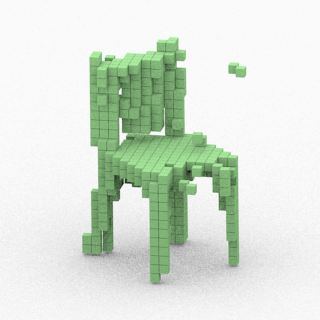
\includegraphics[width=.166\linewidth]{prgan/fig/interpolation/ch7.png} \\
\end{tabular}
\caption{\label{prgan:interp} Shape interpolation by linearly interpolating the encodings of the starting shape and ending shape.}
\end{figure}

\subsubsection{Shape interpolation}
Once the generator is trained, any encoding $z$ supposedly generates a
plausible 3D shape, hence $z$ represents a 3D shape manifold. Similar
to previous work, we can interpolate between 3D shapes by linearly
interpolating their $z$ codes. Figure~\ref{prgan:interp} shows the
interpolation results for two airplane models and two chair models. 



\begin{figure}[t]
	\centering
	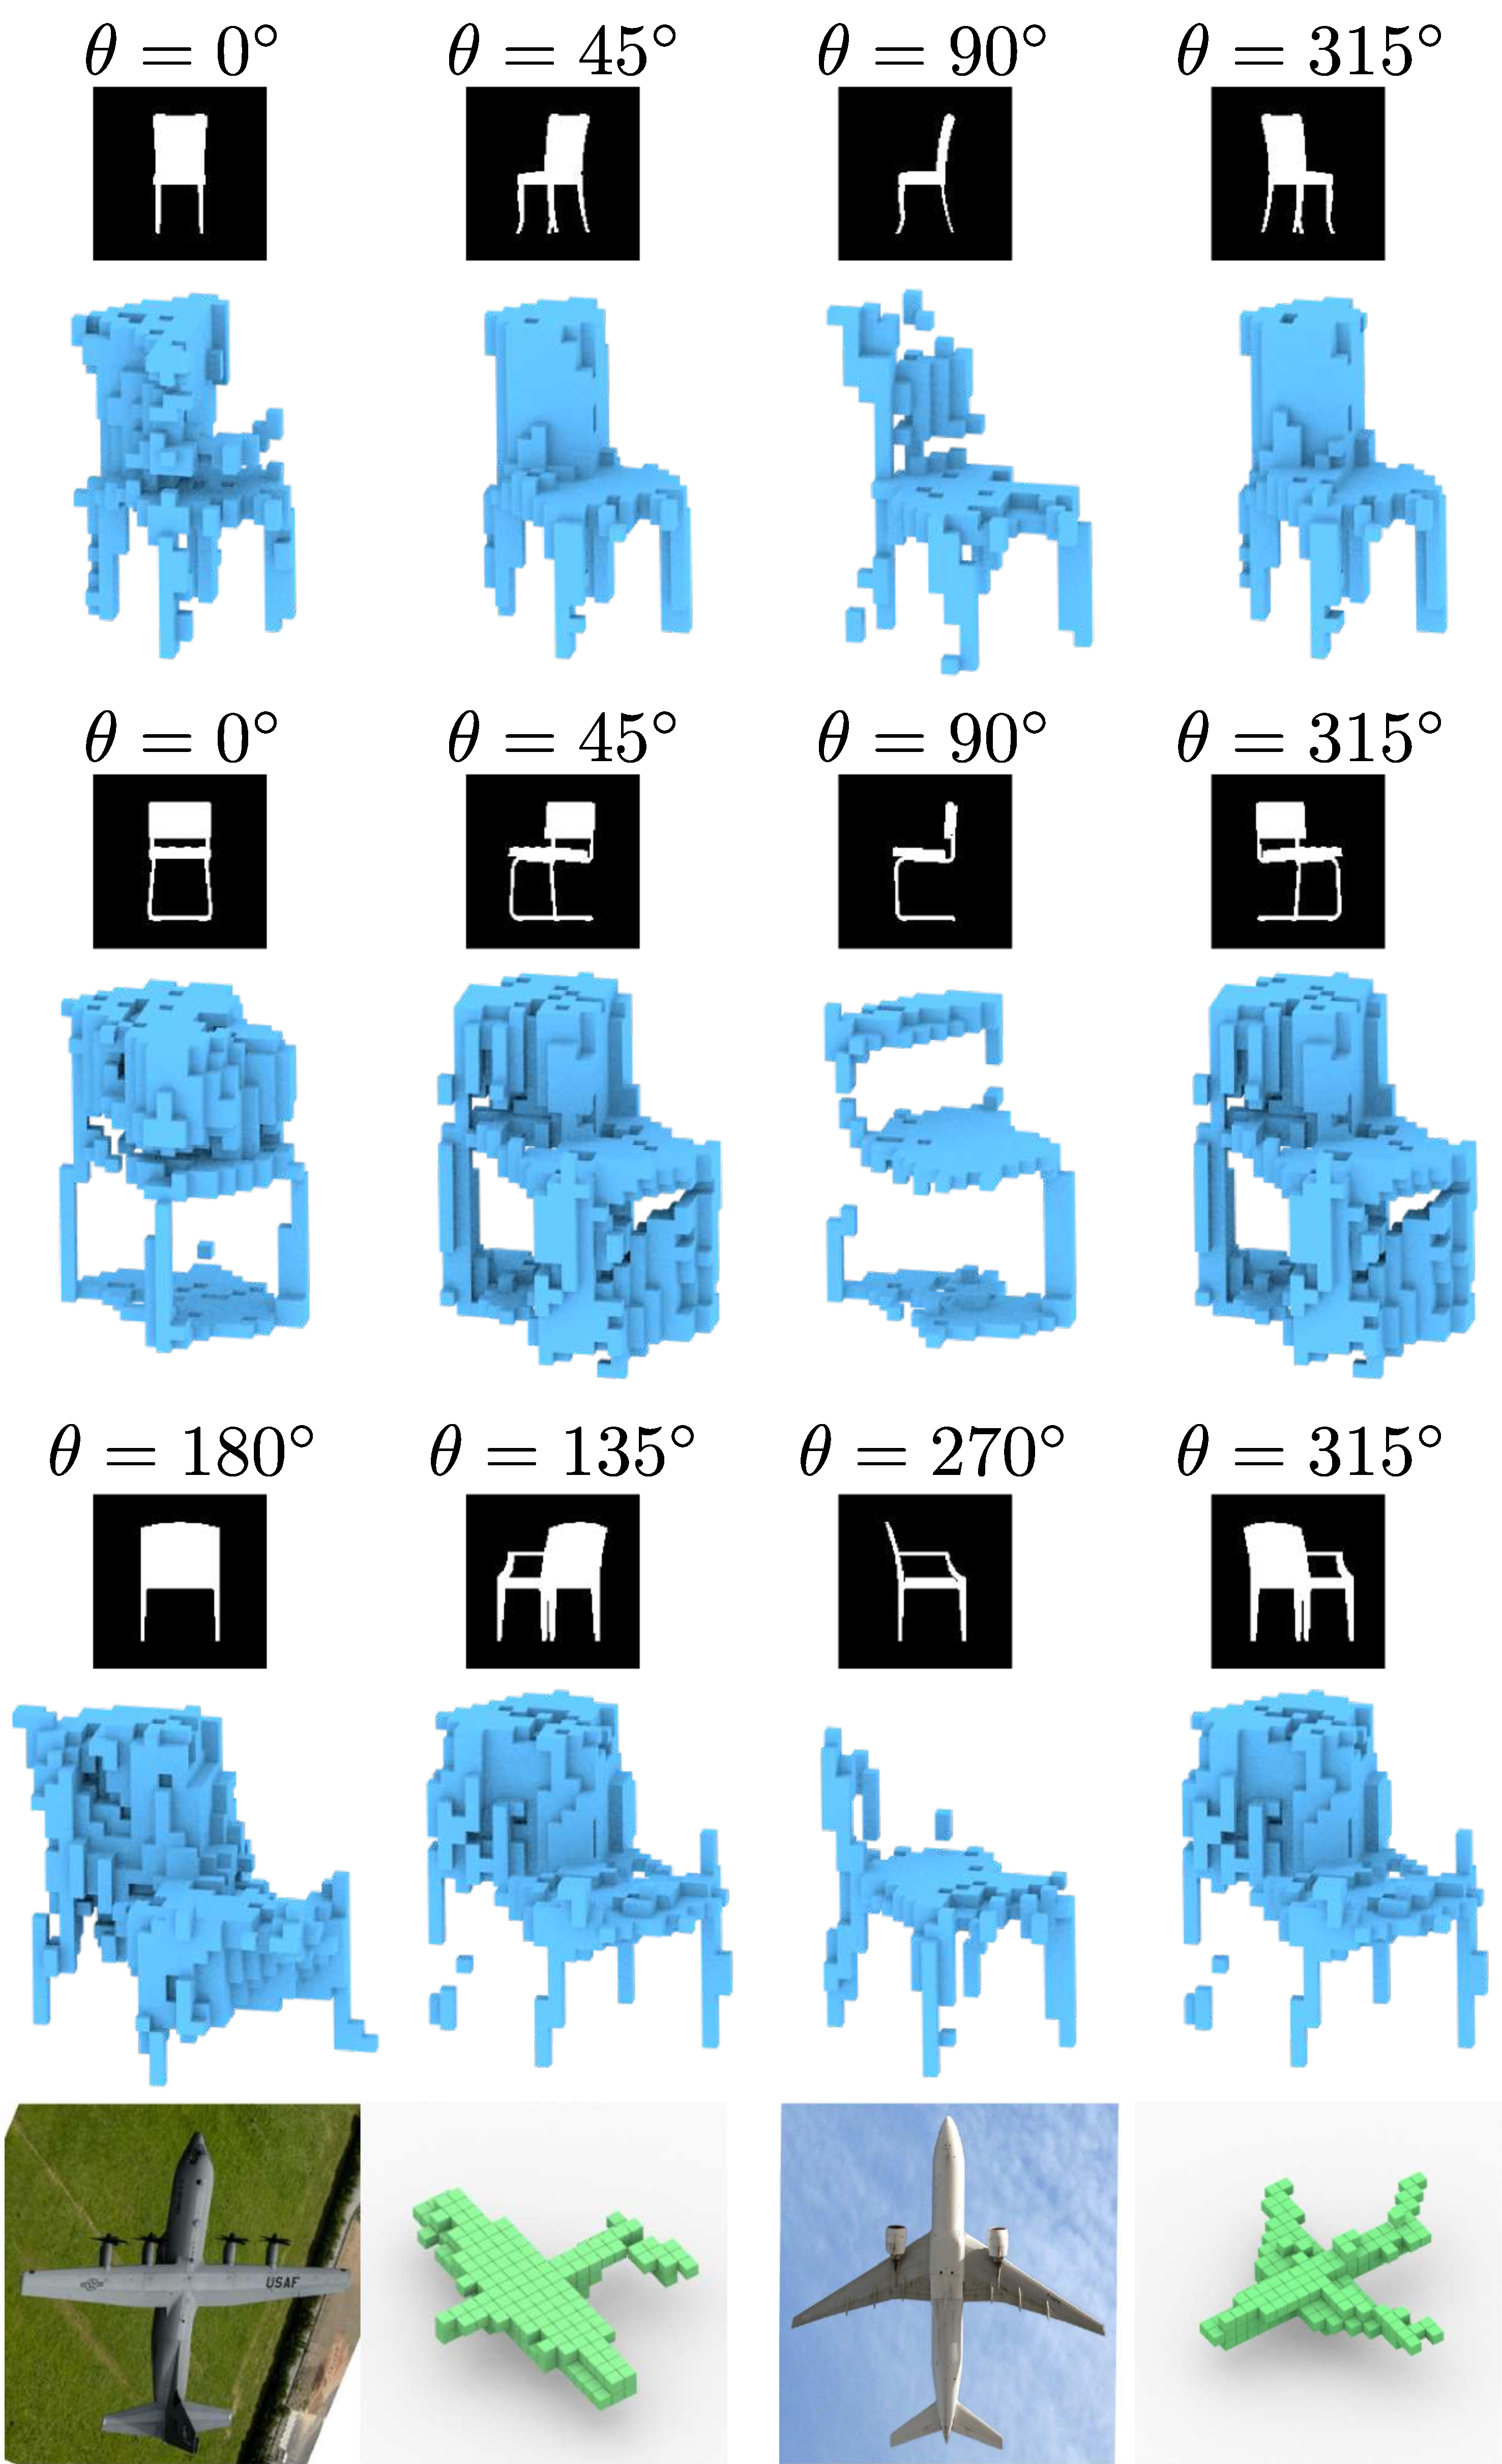
\includegraphics[width=0.85\linewidth]{prgan/fig/shapepred.pdf}
	\caption{\small \label{fig:sp} 
	At top 3 rows, the four images are different views of the same chair, with predicted viewpoint on the top. 
	Shapes are different but plausible given the single view.
	In the bottom row, shape inferred (right) by a single view image (left) using the encoding network. 
	Input images were segmented, binarized and resized to match the network input.}
\end{figure}



\subsubsection{Unsupervised shape and viewpoint prediction}
Our method is also able to handle unsupervised prediction of shapes in 2D images.
Once trained, the 3D shape generator is capable of creating shapes from
a set of encodings $z \in \mathbb{R}^{201}$.
One application is to predict the encoding of the underlying 3D object given a single view image of the object.
We do so by using the \prgan's generator to produce a large number of
encoding-image pairs, then use the data to train a neural network
(called encoding network). In other words, we create a training set
that consists of images synthesized by the \prgan and the encodings
that generated them. The encoding network is fully connected, with 2
hidden layers, each with 512 neurons.
The input of the network is an image and the output is an encoding.
The last dimension of $z$ describes the view, and the first 200
dimensions describe the code of the shape, which allows us to further
reconstruct the 3D shape as a $32^3$ voxel grid. With the encoding
network, we can present to it a single view image, and it outputs the
shape code along with the viewing angle. 
Experimental results are shown in in Figure~\ref{fig:sp}. This whole
process constitutes a completely unsupervised approach to creating a
model that infers a 3D shape from a single image.

\begin{figure*}[h!]
  \newcommand{\fh}{0.18\linewidth}
  \begin{center}
  \setlength{\tabcolsep}{3pt}
  \begin{tabular}{ccc}
    \textbf{Input} & \textbf{Generated images} & \textbf{Generated shapes} \\
    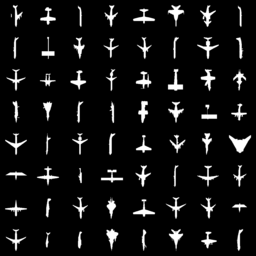
\includegraphics[height=\fh]{prgan/fig/airplane/samples.png} & 
    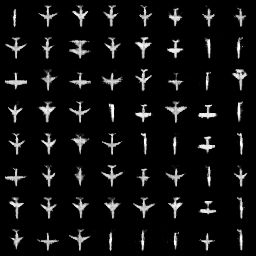
\includegraphics[height=\fh]{prgan/fig/airplane/100.png} & 
    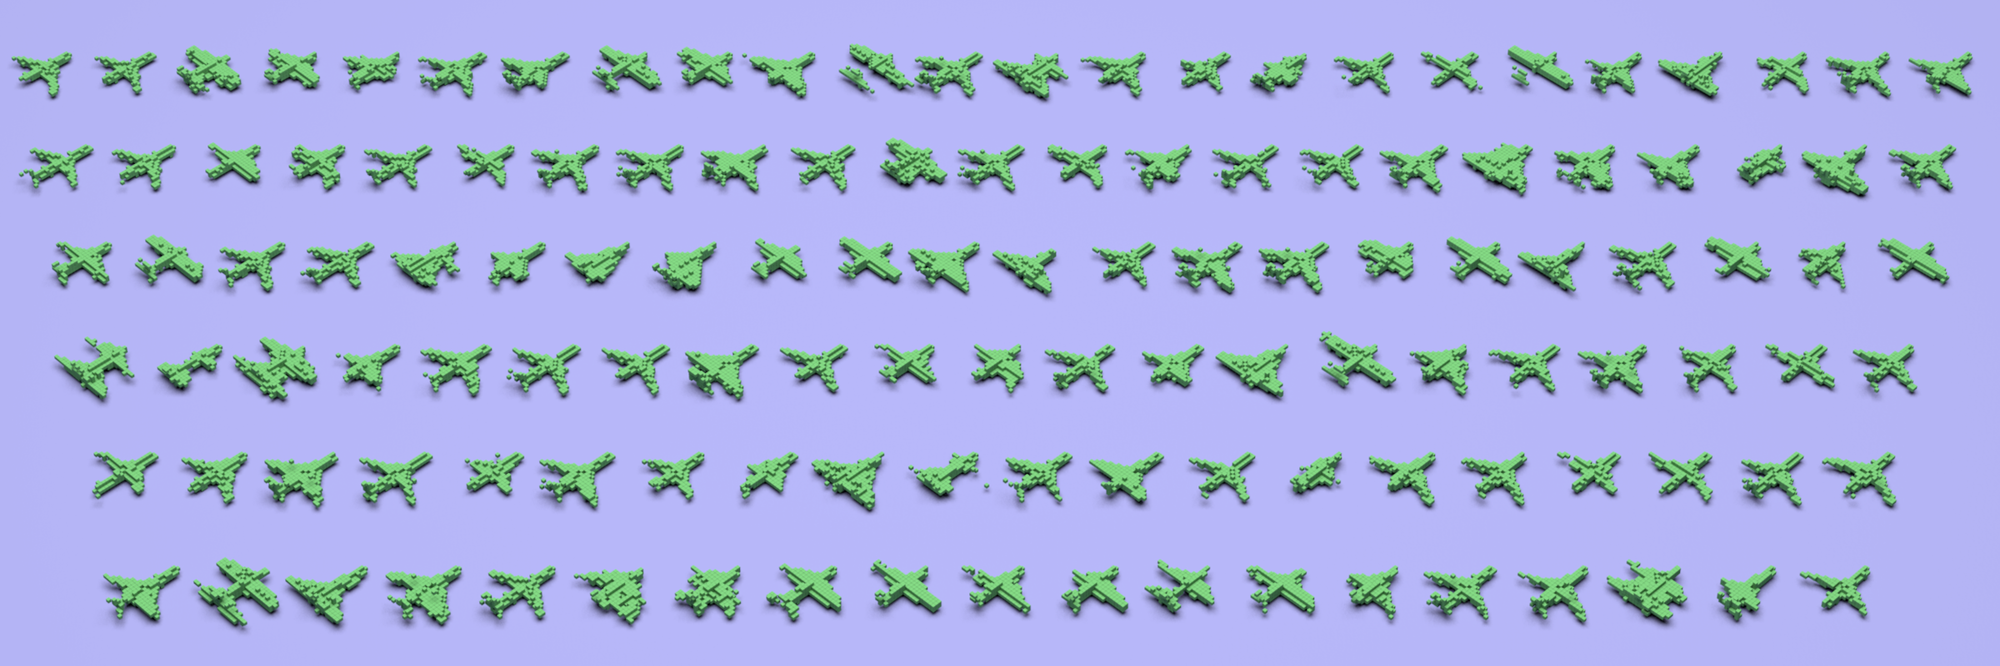
\includegraphics[height=\fh]{prgan/fig/airplane/output.png} \\
    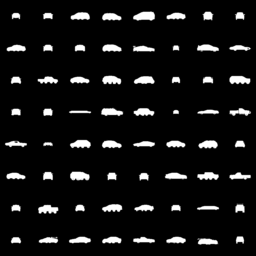
\includegraphics[height=\fh]{prgan/fig/car/samples.png} & 
    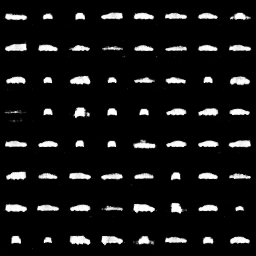
\includegraphics[height=\fh]{prgan/fig/car/600.png} & 
    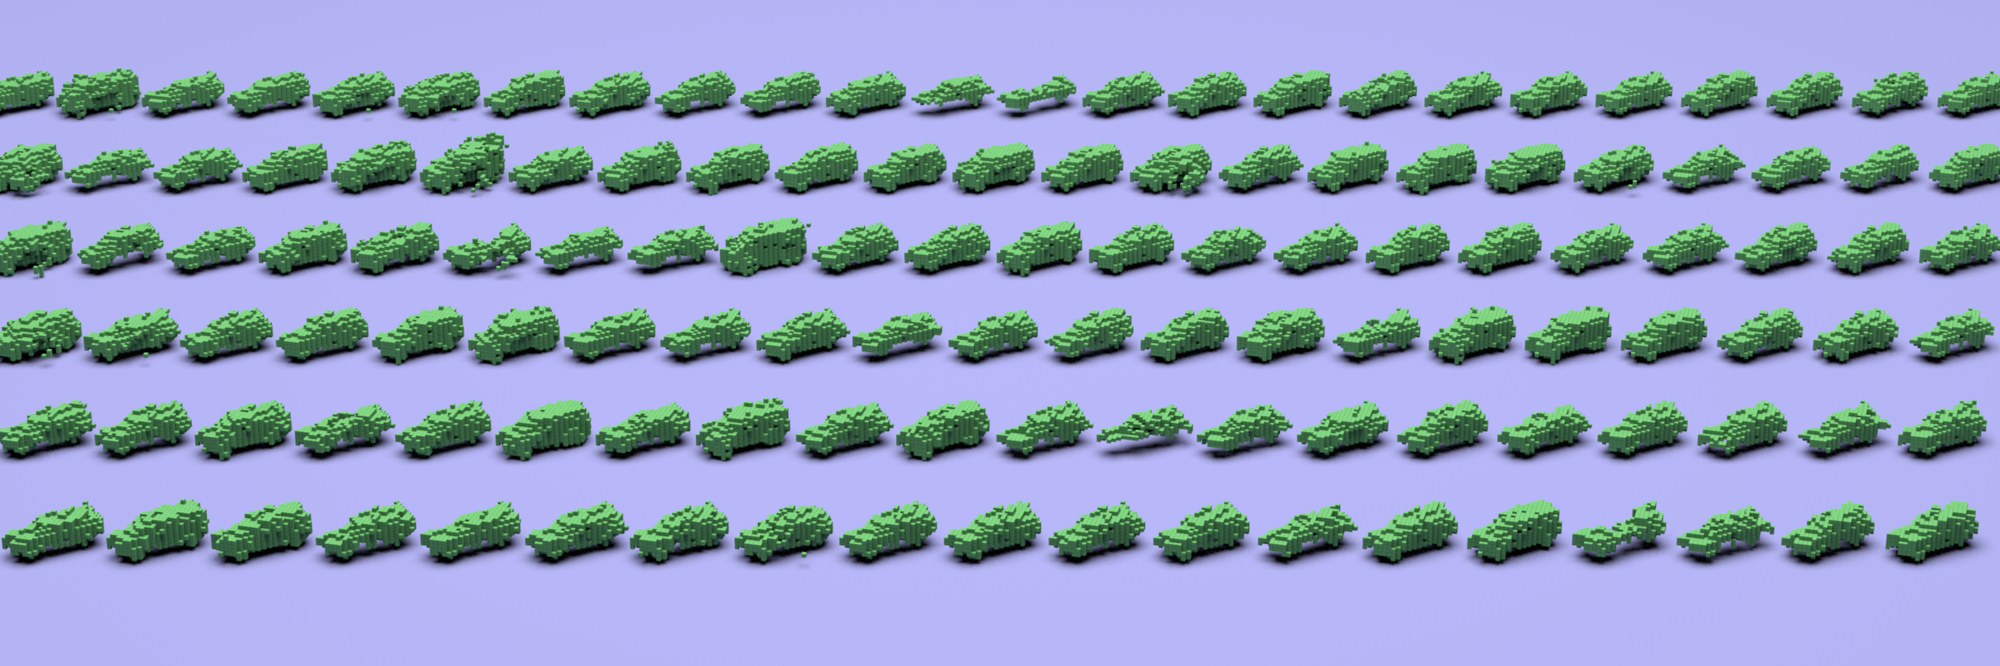
\includegraphics[height=\fh]{prgan/fig/car/output.png} \\
    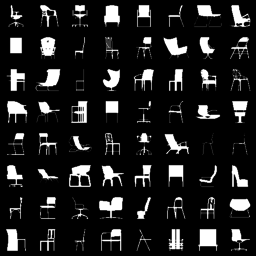
\includegraphics[height=\fh]{prgan/fig/chair/samples.png} & 
    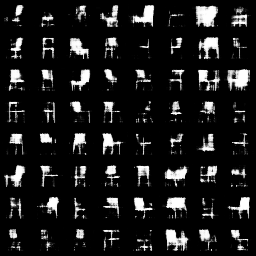
\includegraphics[height=\fh]{prgan/fig/chair/550.png} & 
    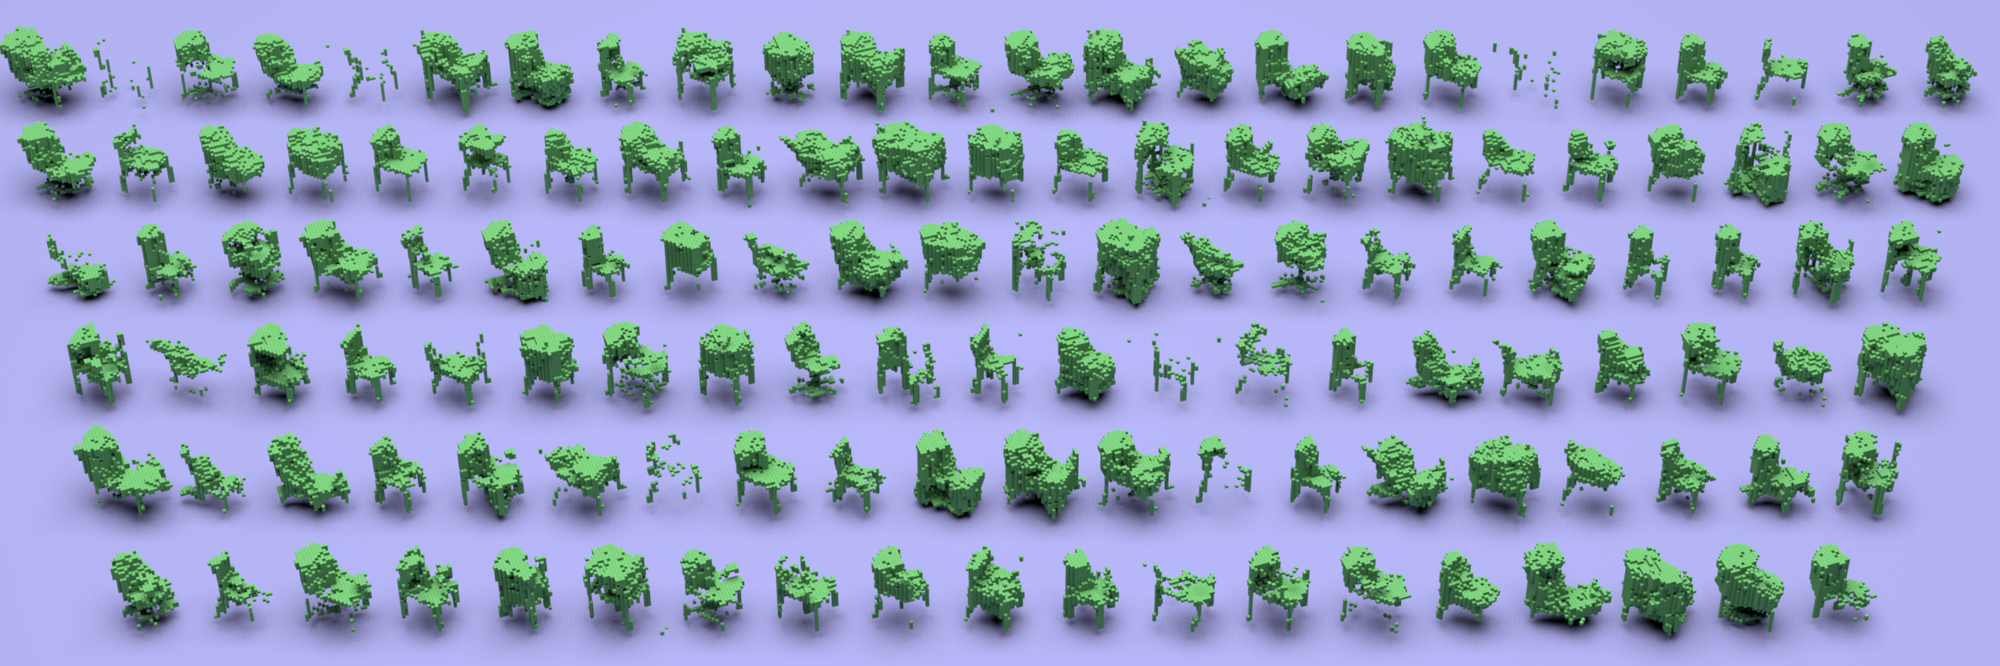
\includegraphics[height=\fh]{prgan/fig/chair/output.png} \\
    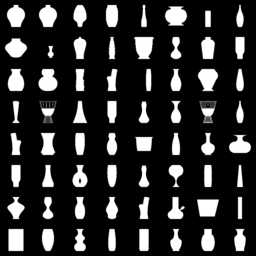
\includegraphics[height=\fh]{prgan/fig/vase/samples.png} & 
    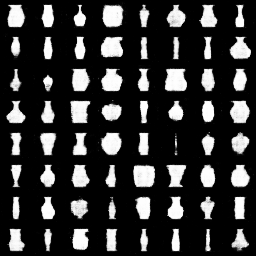
\includegraphics[height=\fh]{prgan/fig/vase/450.png} & 
    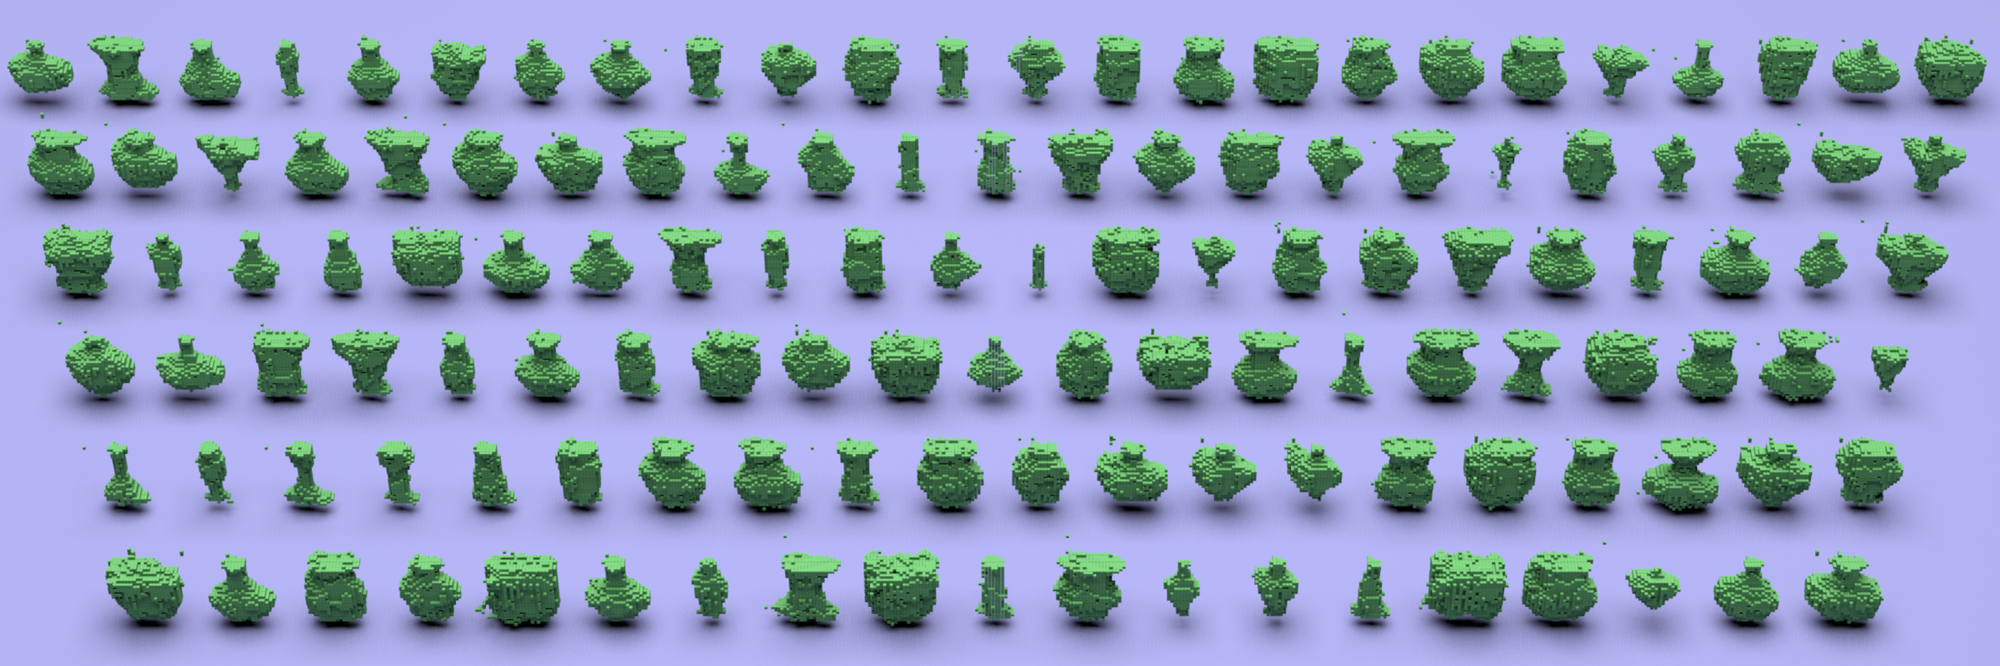
\includegraphics[height=\fh]{prgan/fig/vase/output.png} \\
    \includegraphics[height=\fh]{prgan/fig/bike/samples.png} & 
    \includegraphics[height=\fh]{prgan/fig/bike/300.png} & 
    \includegraphics[height=\fh]{prgan/fig/bike/output.png} \\
    \includegraphics[height=\fh]{prgan/fig/mix/samples.png} & 
    \includegraphics[height=\fh]{prgan/fig/mix/0.png} & 
    \includegraphics[height=\fh]{prgan/fig/mix/output.png} \\
  \end{tabular}
  \end{center}
  \vspace{-6pt}
  \caption{\small \label{fig:generate-shapes} Results for 3D shape induction using \prgans. From top to bottom we show results for airplane, car, chair, vase, motorbike, and a 'mixed' category obtained by combining training images from airplane, car, and motorbike. In each row, we show on the left 64 randomly sampled images from the input data to the algorithm, on the right 128 sampled 3D shapes from \prgan, and in the middle 64 sampled images after the projection module is applied to the generated 3D shapes. The model is able to induce a rich 3D shape distribution for each category. The mixed-category produces reasonable 3D shapes across all three combined categories. Zoom in to see details.}
\end{figure*}

\begin{figure*}[t]
\centering
\setlength{\tabcolsep}{0pt}
\begin{tabular}{cccccccccc}
\includegraphics[width=.1\linewidth]{prgan/fig/airplane/sel0009.png} &
\includegraphics[width=.1\linewidth]{prgan/fig/airplane/sel0012.png} &
\includegraphics[width=.1\linewidth]{prgan/fig/airplane/sel0007.png} &
\includegraphics[width=.1\linewidth]{prgan/fig/airplane/sel0003.png} &
\includegraphics[width=.1\linewidth]{prgan/fig/airplane/sel0002.png} &
\includegraphics[width=.1\linewidth]{prgan/fig/airplane/sel0004.png} &
\includegraphics[width=.1\linewidth]{prgan/fig/airplane/sel0006.png} &
\includegraphics[width=.1\linewidth]{prgan/fig/airplane/sel0008.png} &
\includegraphics[width=.1\linewidth]{prgan/fig/airplane/sel0001.png} &
\includegraphics[width=.1\linewidth]{prgan/fig/airplane/sel0011.png} \\
\includegraphics[width=.1\linewidth]{prgan/fig/car/sel0010.png} &
\includegraphics[width=.1\linewidth]{prgan/fig/car/sel0005.png} &
\includegraphics[width=.1\linewidth]{prgan/fig/car/sel0001.png} &
\includegraphics[width=.1\linewidth]{prgan/fig/car/sel0004.png} &
\includegraphics[width=.1\linewidth]{prgan/fig/car/sel0002.png} &
\includegraphics[width=.1\linewidth]{prgan/fig/car/sel0006.png} &
\includegraphics[width=.1\linewidth]{prgan/fig/car/sel0007.png} &
\includegraphics[width=.1\linewidth]{prgan/fig/car/sel0012.png} &
\includegraphics[width=.1\linewidth]{prgan/fig/car/sel0011.png} &
\includegraphics[width=.1\linewidth]{prgan/fig/car/sel0008.png} \\
\includegraphics[width=.1\linewidth]{prgan/fig/vase/sel0013.png} &
\includegraphics[width=.1\linewidth]{prgan/fig/vase/sel0003.png} &
\includegraphics[width=.1\linewidth]{prgan/fig/vase/sel0011.png} &
\includegraphics[width=.1\linewidth]{prgan/fig/vase/sel0015.png} &
\includegraphics[width=.1\linewidth]{prgan/fig/vase/sel0001.png} &
\includegraphics[width=.1\linewidth]{prgan/fig/vase/sel0014.png} &
\includegraphics[width=.1\linewidth]{prgan/fig/vase/sel0016.png} &
\includegraphics[width=.1\linewidth]{prgan/fig/vase/sel0002.png} &
\includegraphics[width=.1\linewidth]{prgan/fig/vase/sel0005.png} &
\includegraphics[width=.1\linewidth]{prgan/fig/vase/sel0007.png} \\
\includegraphics[width=.1\linewidth]{prgan/fig/bike/sel0006.png} &
\includegraphics[width=.1\linewidth]{prgan/fig/bike/sel0005.png} &
\includegraphics[width=.1\linewidth]{prgan/fig/bike/sel0008.png} &
\includegraphics[width=.1\linewidth]{prgan/fig/bike/sel0004.png} &
\includegraphics[width=.1\linewidth]{prgan/fig/bike/sel0007.png} &
\includegraphics[width=.1\linewidth]{prgan/fig/bike/sel0010.png} &
\includegraphics[width=.1\linewidth]{prgan/fig/bike/sel0009.png} &
\includegraphics[width=.1\linewidth]{prgan/fig/bike/sel0003.png} &
\includegraphics[width=.1\linewidth]{prgan/fig/bike/sel0002.png} &
\includegraphics[width=.1\linewidth]{prgan/fig/bike/sel0001.png} 
\end{tabular}
\caption{\label{fig:example-samples} A variety of 3D shapes generated by  \prgan trained on 2D views of (from the top row to the bottom row) airplanes, cars, vases, and bikes. These examples are chosen from the gallery in Figure~\ref{fig:generate-shapes} and demonstrate the quality and diversity of the generated shapes.}\end{figure*}

\begin{figure}[t]
\centering
\includegraphics[width=0.9\linewidth]{prgan/fig/failure.png}
\caption{\label{fig:failure} Our method is unable to capture the concave interior structures in this chair shape. The pink shapes show the original shape used to generate the projected training data, shown by the three binary images on the top (in high resolution). The blue voxel representation is the inferred shape by our model. Notice the lack of internal structure.}
\end{figure}

\subsubsection{Visualizations across categories} 
Our method is able to generate 3D shapes for a wide range of
categories. 
Figure~\ref{fig:generate-shapes} show a gallery of results,
including airplanes, car, chairs, vases, motorbikes. For each category
we show 64 randomly sampled training images, 64 generated images from
\prgan, and renderings of 128 generated 3D shapes (produced by randomly
sampling the 200-d input vector of the generator). 
One remarkable property is that the generator produces 3D shapes in a
consistent horizontal and vertical axes, even though the training data
is only consistently oriented along the vertical axis. Our hypothesis
for this is that the generator finds it more efficient to generate
shapes in a consistent manner by sharing parts across
models. Figure~\ref{fig:example-samples} shows selected examples from
Figure~\ref{fig:generate-shapes} that demonstrates the quality and
diversity of the generated shapes. 

The last row in Figure~\ref{fig:generate-shapes} shows an example of a
``mixed'' category, where the training images combine the three
categories of airplane, car, and motorbike. The same \prgan network is
used to learn the shape distributions. Results show that \prgan learns
to represent all three categories well, without any additional
supervision.

\FloatBarrier

\subsection{Failure cases} 
Compared to 3D-GANs, the proposed \prgan models cannot discover structures that are hidden
due to occlusions from all views. For example, it fails to discover that some chairs have concave interiors and the generator simply fills these since it does not change the silhouette from any view as we can see at Figure
\ref{fig:failure}. 
However, this is a natural drawback of view-based approaches since
some 3D ambiguities cannot be resolved (\eg, Necker cubes) without
relying on other cues. Despite this, one advantage over 3D-GAN is that
our model does not require consistently aligned 3D shapes since it
reasons over viewpoints.
